% ******************************* Thesis Appendix B ********************************

\chapter{Desaf\'ios t\'ecnicos encontrados}

% **************************** Define Graphics Path **************************
\ifpdf
    \graphicspath{{Appendix2/Figs/Raster/}{Appendix2/Figs/PDF/}{Appendix2/Figs/}}
\else
    \graphicspath{{Appendix2/Figs/Vector/}{Appendix2/Figs/}}
\fi

Durante toda la ejecuci\'on del proyecto, nos enfrentamos a desaf\'ios y en particular de carácter t\'ecnico. Dentro de estos desaf\'ios podemos encontrar algunos que se destacan por su complejidad y dificultad para resolverlos; y otros que se destacan por su severidad como riesgo tecnol\'ogico dentro del proyecto. Por ello consideramos apropiado incluir un ap\'endice para hacer menci\'on a los mismos y a sus respectivas resoluciones.

\section{Problemas con SFPs y Patchcoords}

Los tranceptores SFP+ o transceivers SFP+, son una componente de hardware utilizados en cada puerto f\'isico de la tarjeta NetFPGA en el protot\'ipo.\\ 
 
Or\'iginalmente se trabajo con dos tranceptores SFP+ y patchords de f\'ibra \'optica monomodo. En este punto el hardware funcionaba correctamente. Luego se incorporaron m\'as unidades de SFP+ con el objetivo de constru\'ir el testbed mencionado en [linik a la secci\'on de pruebas donde se presenta el testbed]. En este caso se detectaron problemas para establecer conexiones exitosas para cualquier par de nodos en que se utilizara al menos uno de los SFP nuevos.\\

Tras varias pruebas que confirmaran el error, se consulto con la documentaci\'on y con el equipo generado con ANTEL. Tras la sugerencia de utilizar fibra multimodo en vez de monomodo se logro establecer conexiones exitosas entre todos los pares de interfaces del hardware.\\

Como conclusi\'on general, para el hardware utilizado se debe utilizar patchcords de fibra multimodo.


\section{Desprogramaci\'on del hardware NetFPGA}
\label{apendiceB2}

Para la programación del hardware NetFPGA, se utiliza inicialmente el procedimiento indicado en el manual de ejecuci\'on del Test de Producci\'on ~\citep{ProdTestManual}. Tras experimentarse un tiempo con este procedimiento y el hardware se constata que esta técnica de programación no es persistente. Esto significa que tras apagar y encender el equipo(ciclo completo de encendido) el mismo pierde la programación. 

Utilizando la herramienta Impact, observando el comportamiento de LEDs en la placa y corroborando con el el manual de la misma, se constata que el contenido del chip CPLD no es borrado, pero el del chip FPGA si.\\

Con esta información se consulta la documentación de la plataforma, y se buscan experiencias similares por partes de otros usuarios de la misma. No se encuentran problemas o experiencias similares, pero se encuentra dentro de los proyectos de la plataforma un desarrollo de nombre Reference Flash, cuya funcionalidad es habilitar la programación persistente del hardware.\\

Este proyecto utiliza las dos unidades de memoria flash del equipo. Mientras que en la Flash A se almacena un bitstream de configuración para el equipo (bootstrap bitstream), la  Flash B queda disponible para almacenar un bitstream a elección del programador. 

La configuración del equipo es siempre manejada por el chip CPLD, el cual en el tiempo de encendido programa al equipo con el contenido de la Flash A. Luego el equipo puede ser reprogramado desde la Flash B a través de la interfaz PCIe.

Basándose en este proyecto, se prueba como solución al problema de la desprogramacion del equipo esta alternativa, utilizando como bitstream para la Flash B, el proyecto ReferenceNIC.\\

Esta estrategia funciona en relación a la desprogramacion del hardware, puesto que tal como su documentación lo indica se programa a partir del contenido de la Flash A; y luego utilizando la interfaz PCIe es existosamente reprogramada desde la Flash B. No obstante el comportamiento final del hardware no es el correcto. En particular tras reprogramar el equipo desde la Flash B no se puede insertar el driver para el ReferenceNIC en el kernel del sistema operativo(Linux).\\

Finalmente se utiliza una lista de correos en la que participan usuarios y desarrolladores de la plataforma. Aquí se explica el problema de la desprogrmacion del hardware, y las alternativas exploradas (ver anexo [link al anexo con el email]). 

Afortunadamente, por parte del equipo de desarrolladores de NetFPGA se nos contesta que este comportamiento se debe a una incorrecta programacion del hardware. Si bien se entiende correctamente la funcionalidad del proyecto ReferenceFlash, el proyecto ReferenceNIC precisa de módulos adicionales en el diseño de la CPLD que el ReferenceFlash no tiene. 

Sin embargo, el proyecto ReferenceNIC ya tiene incorporado el modulo de persistencia que se presenta en ReferenceFlash. Para lograr una programacion persistente, ademas de programar el equipo con el ReferenceNIC, se debe utilizar la herramienta \textbf{pcieprog}(dentro del mismo proyecto), para cargar en la memoria Flash A, un archivo bitstream con el contenido del mismo proyecto. De esta forma al producirse el encendido del equipo, este se programa con el contenido de la memoria Flash A.\\ 

Esta es la solución al problema de la desprogramacion del hardware, y es lo que se da a conocer en este trabajo como la estrategia de programación persistente.

\section{Falta de licencias para suite de Xilinx ISE SDK}
\label{apendiceB3}

La suite de Xilinx ISE SDK, se componen por un conjunto extenso de herramientas y entornos de desarrollo. Dentro de la suite se encuentran herramientas habilitadas para su uso bajo licencias gratuitas, otras bajo licencias de prueba (tipicamente 30 dias), y otras solamente bajo licencias pagas.\\

En particular en este proyecto se comienza trabajando con un paquete de licencias gratuitas. Seguir explicando \dots\\


Por otro lado, esta estrat\'egia de programaci\'on utiliza herramientas de la suite de Xilinx que requieren de licencias pagas. Este detalle se constato experimentalmente en la ejecuci\'on del proyecto. Cabe destacar que la informaci\'on de error proporcionada por la herramienta al intentar ejecutarla sin las licencias correspondientes, asi como la documentaci\'on disponible no suguieren de forma intuitiva un problema de licencias. Por ello, teniendo la intuici\'on de que se trataba efectivamente de un problema de licenciamiento se solicitaron licencias adicionales a trav\'es del programa de apoyo universitario de Xilinx.

Tras pasar varias semanas a la espera de una respuesta, se establecio un contacto con docentes del IIE de Facultad de Ingenieria. Desde el IIE se contesto que no trabajaban con esta plataforma pero que lo hab\'ian hecho en un pasado; facilit\'andonos un conjunto de licencias con el que se logro resolver el problema de licenciamiento. 

Mucho tiempo despu\'es el programa universitario de Xilinix don\'o un paquete de licencias entre las cuales se encontraban las necesarias. Por m\'as detalles acerca de este problema referirse al siguiente ap\'endice [link al apendice y problema tecnico].

\section{Falta de driver para cable JTAG Xilinx}
Si mal no recuerdo tuvimos algun problema en relacion a esto. Tengo la vaga idea de que yo queria usar algo de linux que te permite correr drivers no recuerdo si viejos.... Fa capaz me estoy mareando con lo de la wireless de asus.

\section{Desaf\'ios con Open vSwitch}
\label{apendiceB5}

Open vSwitch es uno de los pilares fundamentales del router opensource, puesto que es el encargado de implementar el plano de datos de OpenFlow. Durante el tiempo en que se trabaj\'o con esta herramienta se genero experiencia y conocimiento en relaci\'on aspectos importantes sobre esta herramienta, que no son triviales y vale la pena mencionar.\\ 

\begin{enumerate}
\item Parte de las funcionalidades de Open vSwitch, est\'an implementadas para funcionar en modo kernel, y parte en modo usuario. Estas \'ultimas presentan un nivel de performance muy pobre en comparaci\'on a la primera; y en particular las funcionalidades de MPLS se encuentran solamente disponibles en modo usuario.

\item De acuerdo a las notas de liberaci\'on de la \'ultima versi\'on oficial de Open vSwitch(2.3.1), 
esta garantizado el soporte a MPLS en las operaciones de match, push y pop, para una \'unica etiqueta, as\'i como el posterior procesamiento del paquete de acuerdo al pipe de OpenFlow, funcionando en modo usuario.

\item Originalmente las notas de liberaci\'on de Open v Switch v2.3.1, y la p\'agina de preguntas frecuentes no se correspond\'ian con el comportamiento del software. En particular se garantizaba el soporte para match, push, pop y posterior procesamiento de un paquete MPLS en una \'unica etiqueta.
Experimentalmente se comprobo que las operaciones de match y push funcionaban correctamente para una \'unica etiqueta. No obstante la operaci\'on de POP no estaba soportada. Este comportamiento fue detectado y reportado por otros usuarios de Open vSwitch, resolviéndose posteriormente en la versi\'on de desarrollo de Open vSwitch~\citep{OVSSourceCode}.

\item Trabajando con la versi\'on m\'as del HEAD, en el repositorio de desarrollo de Open vSwitch~\citep{OVSSourceCode}, se comprueba experimentalmente el soporte para las operaciones de match, push y pop de hasta 3 etiquetas, y el posterior procesamiento del paquete seg\'un el pipe de procesamiento de OpenFlow.

\item Puertos OpenFlow con direcciones IP
%Una condici\'on necesaria en la arquitectura del prototipo es la capacidad de asignar direcciones IP a cada interaz del router opensource.
 
Para lograr que cada interfaz f\'isica de la tarjeta NetFPGA se comporte tanto como un puerto OpenFlow, como una interfaz IP, es necesario:

\begin{enumerate}
\item Crear un bridge con Open vSwitch, y agregar cada interaz f\'isica como un puerto OpenFlow al mismo.
\item Asignar una dirección IP a la propia intefaz f\'isica (por ejemplo utilizando el comando ifconfig).
\end{enumerate}

%Debido al comportamiento de un bridge en Linux, esta estrategia que parece natural e inmediata, no se comporta en la pr\'actica como se necesita en este proyecto. El comportamiento deseado de una interfaz h\'ibrida IP/OpenFlow en el prototipo ser\'ia el que se indica en la figura~\ref{fig:OVSInterfaces}.

El comportamiento deseado por una interfaz h\'ibrida IP/OpenFlow en el prototipo ser\'ia el que se muestra en la figura ~\ref{fig:OVSInterfaces} parte izquierda.

El paquete ingresa al router atrav\'es de la interfaz f\'isica \textbf{nf0} y de ah\'i en m\'as el procesamiento del mismo es delegado al m\'odulo de Open vSwitch en el kernel de Linux. Aqu\'i el paquete es procesado y tratado en consecuencia a lo que indica la tabla de flujos en Open vSwitch. En el prototipo, para este paquete existen dos alternativas: (1) se procesa el contenido del mismo y se reenv\'ia por otra interfaz acorde a la regla correspondiente, (2) es contemplado por una regla con la acci\'on \textit{NORMAL}, y por tanto es procesado como lo har\'ia un switch legado(en este caso como lo procesar\'ia el kernel de linux).\\

No obstante, el procesamiento del paquete al ingresar por la interfaz f\'isica \textbf{nf0} difiere(ver parte derecha de imagen). El paquete es procesado por Open vSwitch como se describi\'o anteriormente, pero tambi\'en es enviado para su procesamiento en el kernel de linux.

Esto implica que el router se comporte tanto como un switch OpenFlow como un equipo tradicional. Como este comportamiento es inaceptable dentro del prototipo, se debe buscar una solución a dicho problema.

\begin{figure}[htbp!] 
\centering    
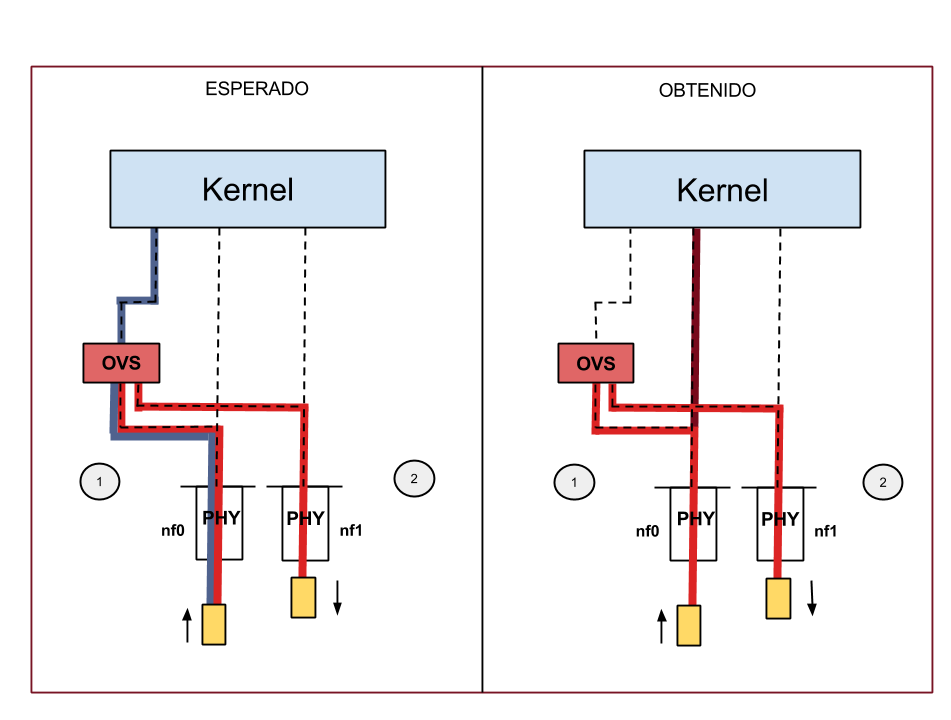
\includegraphics[width=0.75\textwidth]{ovs_figure3}
\caption[OVSInterfaces]{Descripci\'on esquematica de interfaces propuesta}
\label{fig:OVSInterfaces}
\end{figure}

Para solucionar este problema se utilizan interfaces virtuales. Ficha por favor como seguimos aca\dots...

\begin{figure}[htbp!] 
\centering    
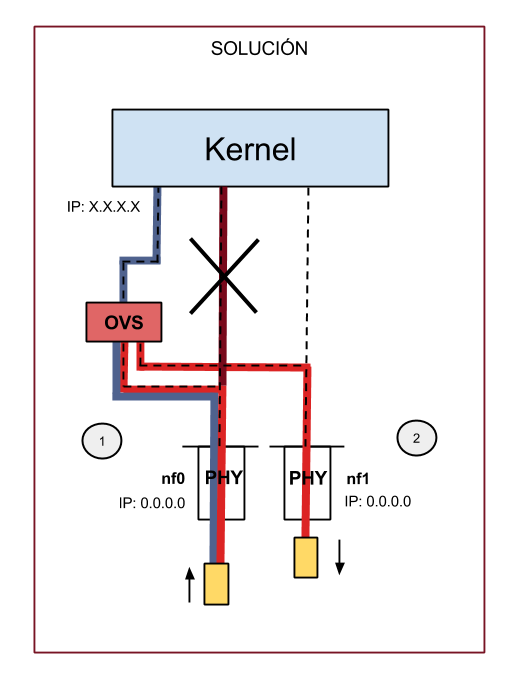
\includegraphics[width=0.40\textwidth]{ovs_figure4}
\caption[OVSInterfaces2]{Descripci\'on esquematica de interfaces propuesta}
\label{fig:OVSInterfaces2}
\end{figure}


\end{enumerate}

\section{MPLS Linux y Quagga LDP}
Bueno creo que es aca donde sacarnos las ganas de hablar de Quagga LDP y MPLS linux

Que es MPLS LINUX, las dos versiones que hay, que es quagga LDP las dos versiones que hay.

Con que se empezo, que problemas tuvimos. Poca documentacion o practicamente nada.

Se recompila kernel, cambia configuracion, se logra configuracion intermedia.

La version original de MPLS Linux, no andaba porque no soportaba openvswitch, no reconocia la placa etc.

Ademas no compilaba la version que estaba en repositorio. Tenia errores de compilacion, faltaban herramientas para instalar que no existian. Muchos pero muchos problemas tecnicos.

Se probaron kernels desde la 3.09.algo hasra la 3.11.26 creo generic, a unas versiones mas viejas. En la confuguracion del kernel no estaba disponible MPLS, Openvswitch, un asco todo.

Se logor hacer andar el MPLS linux nuevo con el LDP nuevo.

Se podian insertar cosas en las tablas de MPLS y el quagga por si solo andaba. No obstante no funcionaba que se insertaran desde el LDP cosas a las tablas MPLS. En particular se moria cuando intentaba insertar la primer entrada de MPLS asociada a la tabla FTN para una fec en particualr. Debugueamos el codigo, inspeccionamos y acorralamos el bug pero no pudimos solucionarlo. Se co nsidero una perdida de tiempo asi que se siguio.

[make menuconfig]

\section{Instalaci\'on de Sistema Operativo}
Instalamos Fedora 14 y no booteaba. Desactivamos el uefi de la bios y tampoco. Probamos con varias versiones de Fedora incluso con un dvd de la uri y descargada de internet. Probamos con dvd y usb.

Fedeora 20 era compatible con la mother pero no encontrabamos driver para el cable programador.

Logramos instalar Xilinx en window XP SP3 con los drivers del cable. Aqui se podian programar las placas para las pruebas de aceptacion.

Probamos con Ubuntu 14.04, y las placas se reconocian el driver existia pero las pruebas de aceptacion no encaraban (fallaban todas). Problemas con el DMA.

Se probo con Ubuntu 12.04 y se logro instalar Xilinx, conseguir driver, reconocer placa y las pruebas de aceptacion ok!. 